In this section, the results of the benchmark runs will be analyzed and presented.
When discussing the number of threads $N$, this number will include the coordinator thread except where specified.
It was previously discussed that PRS requires each search thread $tid_i$, where $i > 2$ to do two iterations of fringe search. 
In other words, the amount of work doubles once the algorithm is run with more than three threads. 
Taking this into account, the expected speedup of PRS is calculated as follows:

\begin{align*}
    & work = 
    \begin{cases} 
        1 & N \leq 3 \\
        2 & N > 3
    \end{cases} 
    & speedup = \frac{N-1}{work}
\end{align*}

\noindent where $N$ is the total number of threads including the coordination thread. This can be compared to the average runtime as shown in \figref{fig:runtime}. Expected runtime is defined as the quotient of sequential runtime and expected speedup.

\begin{figure}[H]
    \centering
    \includegraphics[width=\linewidth]{img/runtime.eps}
    \caption{Comparative runtime performance on large paths for all relevant algorithm implementations. The expected runtime is based on the corresponding sequential algorithm performance.}
    \label{fig:runtime}
\end{figure}

\noindent For sufficiently large graphs, PRS achieves almost linear speedup up to approximately 8 search threads compared to sequential fringe search. 
The vectorized versions of both fringe search and PRS outperform their counterpart at any given thread count, and as is clear, both PRS and fringe search outperform A*. 
The likely culprit of Boost's \linebreak\lstinline{astar_search} performance deficit is its underlying graph representation. Using a generalized graph seemed to be slightly slower on dense maps and significantly faster on sparse ones, however, as the benchmarks maps are mostly dense, the performance delta to our A* implementation can be easily explained.

\begin{figure}[H]
    \centering
    \includegraphics[width=\linewidth]{img/speedup.eps}
    \caption{Achieved speedup compared to the baseline fringe search for increasingly more \textit{search threads} over all benchmark scenarios.}
    \label{fig:speedup}
\end{figure}

\noindent All algorithm configurations are tested on the same set of benchmarks, thus relying on strong scaling. 
Observing \figref{fig:speedup}, PRS misses the mark with two search threads, where the initialization and coordination overhead seems to outweigh any improvements in search time.
In limited testing with randomly generated graphs containing paths of up to $6,000$ vertices, PRS-12 achieved a peak speedup of $7.4$ compared to fringe search and PRS-24 achieving a speedup of $11$. 
Considering work, this is superlinear and is understandable due to sequential search not being linear in path length. 
In general, it can be expected that the higher the graph's branching factor, the larger the potential advantage for dividing the search into shorter sub-paths.

\mypar{Path Quality}
A fundamental idea behind PRS is to sacrifice path quality for performance. However, the severity of degradation has not been discussed yet.
In terms of path length, all sequential implementations are deterministic. A* is optimal and always finds the shortest possible path.
Vectorized fringe search exhibits a slightly different exploration behavior to its list counterpart, which results in a higher number of explored vertices, and therefore, a closer to optimal path. 
This consequently also translates to vectorized PRS.
PRS exploration behavior is non-deterministic and quality degrades with increasing path length and thread count as seen in \figref{fig:cost-overhead}.
However, $12$ threads still delivered a good balance between performance and quality with our setup.

\begin{figure}[H]
    \centering
    \includegraphics[width=\linewidth]{img/cost_overhead.eps}
    \caption{Mean path cost overhead represented as a percentage of the optimal cost for all benchmark scenarios.}
    \label{fig:cost-overhead}
\end{figure}

\mypar{Consistency}
Lastly, the variance of path length and runtime for each algorithm needs to be assessed. 
As can be seen in \figref{fig:var-time}, adding more threads results in consistently better runtime performance, and surprisingly, PRS runtime was most consistent at very high thread counts.

\begin{figure}[H]
    \centering
    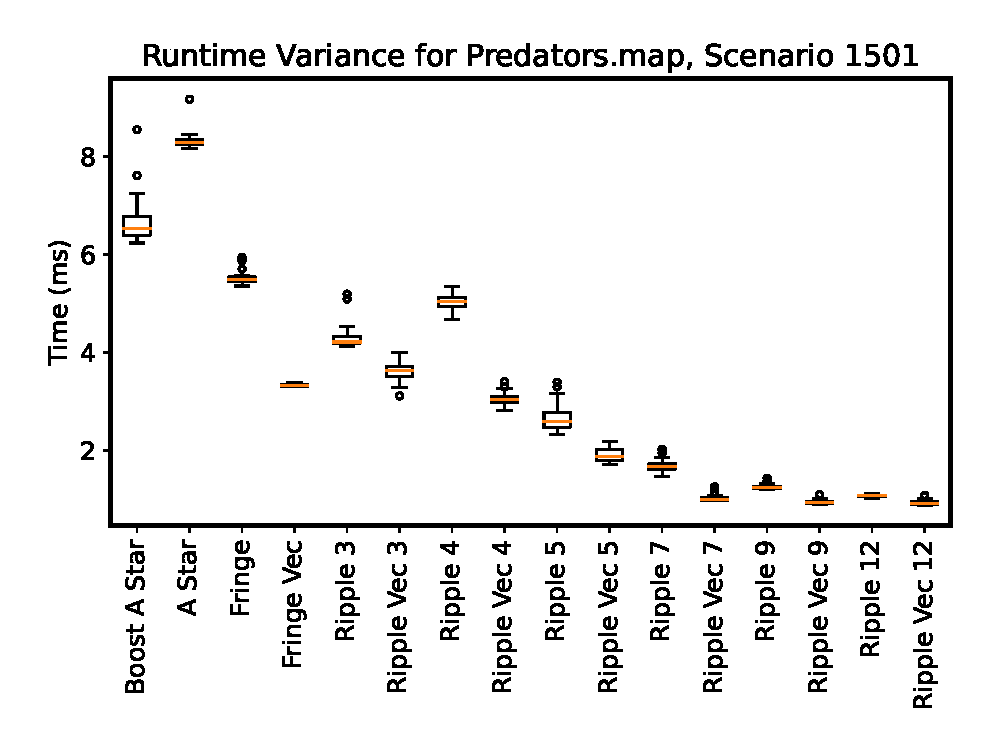
\includegraphics[width=\linewidth]{img/scenario_time.eps}
    \caption{Variability of path length for a representative scenario of the benchmark set, same as used in \figref{fig:ripple_example} and \ref{fig:high}.}
    \label{fig:var-time}
\end{figure}

\noindent Seen in \figref{fig:var-cost}, deterministic search algorithms have zero variance in found path length and PRS length variance increases with the thread count, all as expected.
Over the full run of benchmarks, the variability of each algorithm was low enough in both path length and runtime that further discussion will be omitted, see \figref{fig:var-overall}.
Instead, a decision was made to focus on a hand-picked representative scenario to show consistency in runtime and path quality. 

\begin{figure}[H]
    \centering
    \includegraphics[width=\linewidth]{img/scenario_cost.eps}
    \caption{Variability of path length for a representative scenario of the benchmark set, same as used in \figref{fig:ripple_example} and \ref{fig:high}. The optimal path length is $498$ vertices.}
    \label{fig:var-cost}
\end{figure}

\begin{figure}[h]
    \captionsetup[subfigure]{labelformat=empty}
    \subfloat{
        \includegraphics[width=0.22\textwidth]{img/var_time.eps}
    }
 	\hfill
	\subfloat{
        \includegraphics[width=0.22\textwidth]{img/var_cost.eps}
    }
    \caption{(Left) Variability in total runtime over all benchmark scenarios. (Right) Variability in mean path length over all benchmark scenarios.}
    \label{fig:var-overall}
\end{figure}